\section{Introduction}
In this report, the status update of the CS574 NLP project is presented. An
overview is given of the progress made since the project proposal four weeks
previously. The main work done was to conduct additional literature research,
create a dataset, attempt to implement summarisation algorithms and to evaluate
them. Based on these results, the project will be rounded off in the remaining
two weeks.

\section{Related Work}
Plenty of related work has been discussed earlier sections;~\cite{Gaikwad2016} 
suggests classical approaches of current automatic summarization techniques, 
with plenty of abstractive and extractive methods. Most of early works on 
automatic summarization were focused on documentations for given text, with 
frequency of words and gauging the relateness of each word to given or overall
context. These appearance frequencies are also used in the evaluation.

Recent researches on automatic summarization have approached in statisticall
modelling and machine learning. Naturally those approaches started from the
basic techniques, and so most approaches were made with extractive
methods:~\cite{2017arXiv170804439V}. Since this methodology linterally extract
human language information from given text, the output is the selected subset
of input document. Thus, it is perhaps not possible to paraphrase just like
human, but it was the mainstream of this field. However, this methodology is
highly related to the frequency of word appearance, so that it is challenging
to rank seemingly-important words shown in the input document. Moreover, it is
demanding to understand basic grammar of input language in order to select
subset and reconstruct into several sentences.

As the deep learning approaches became main strategy in many researches areas,
the importance of modelling is risen, many researchers adopt some abstractive
methods in Natural Language
Processing:~\cite{2016arXiv160206023N},~\cite{2017arXiv170404368S},~and~\cite{Rush2015}.
Before, Abstractive sentence summarization has been traditionally used in
headline generation, which gives intuition that abstractive methods is capable
of not only summarizing but also paraphrasing the input documents wich some
understanding of human languages. 

However, most of work on automatic summarization is primarily targeting on
the summarization of article-length input document. It is found that not many
papers are dealing with the input document of book-level length, and most of
those papers are about classification task. This gives us an idea to apply
recent techniques in automatic summarization on books.


\section{Approach}
As it is mentioned, the strategy to summarize whole book should be different
from simply summarizing the article. Word frequency seems it only shows some
main characters, but this informations could possibly be used in abstractive
modelings. 

A dataset was collected from the internet of ten novels and a play, with at
least three summaries each. The books are mainly fictional classics, due to
their popularity on summary resources and often the expiration of their
copyright. Most of the summaries are sourced from CliffsNotes, SparkNotes and
GradeSaver. The books and summaries both vary quite vastly in length. All the
documents were saved as or converted to text files, to facilitate consistency
and ease of manipulation in Python.

\section{Experiments}

\subsection{Algorithms}

Our hypothesis in summarising long texts is that differences between books are
important in the summary. That's why we've analysed the word frequencies in our
set of books. It becomes clear that often the most used, or at least the top 5
noun is referring to the main character. In books where the main character is
named, like \textit{Fahrenheit 451}, or \textit{The Hobbit}, that noun is the
name of the main character. In books where the main character is not named, a
different noun is used, like ``boy'' in \textit{The Alchemist}.

The results of our analysis are contained in the three
graphs~\ref{fig:fahrenheit_451_nouns},~\ref{fig:the_alchemist_nouns},~\ref{fig:the_hobbit_nouns},
which each contain the 30 most used nouns in a book.

\begin{figure}[H]
	\centering
	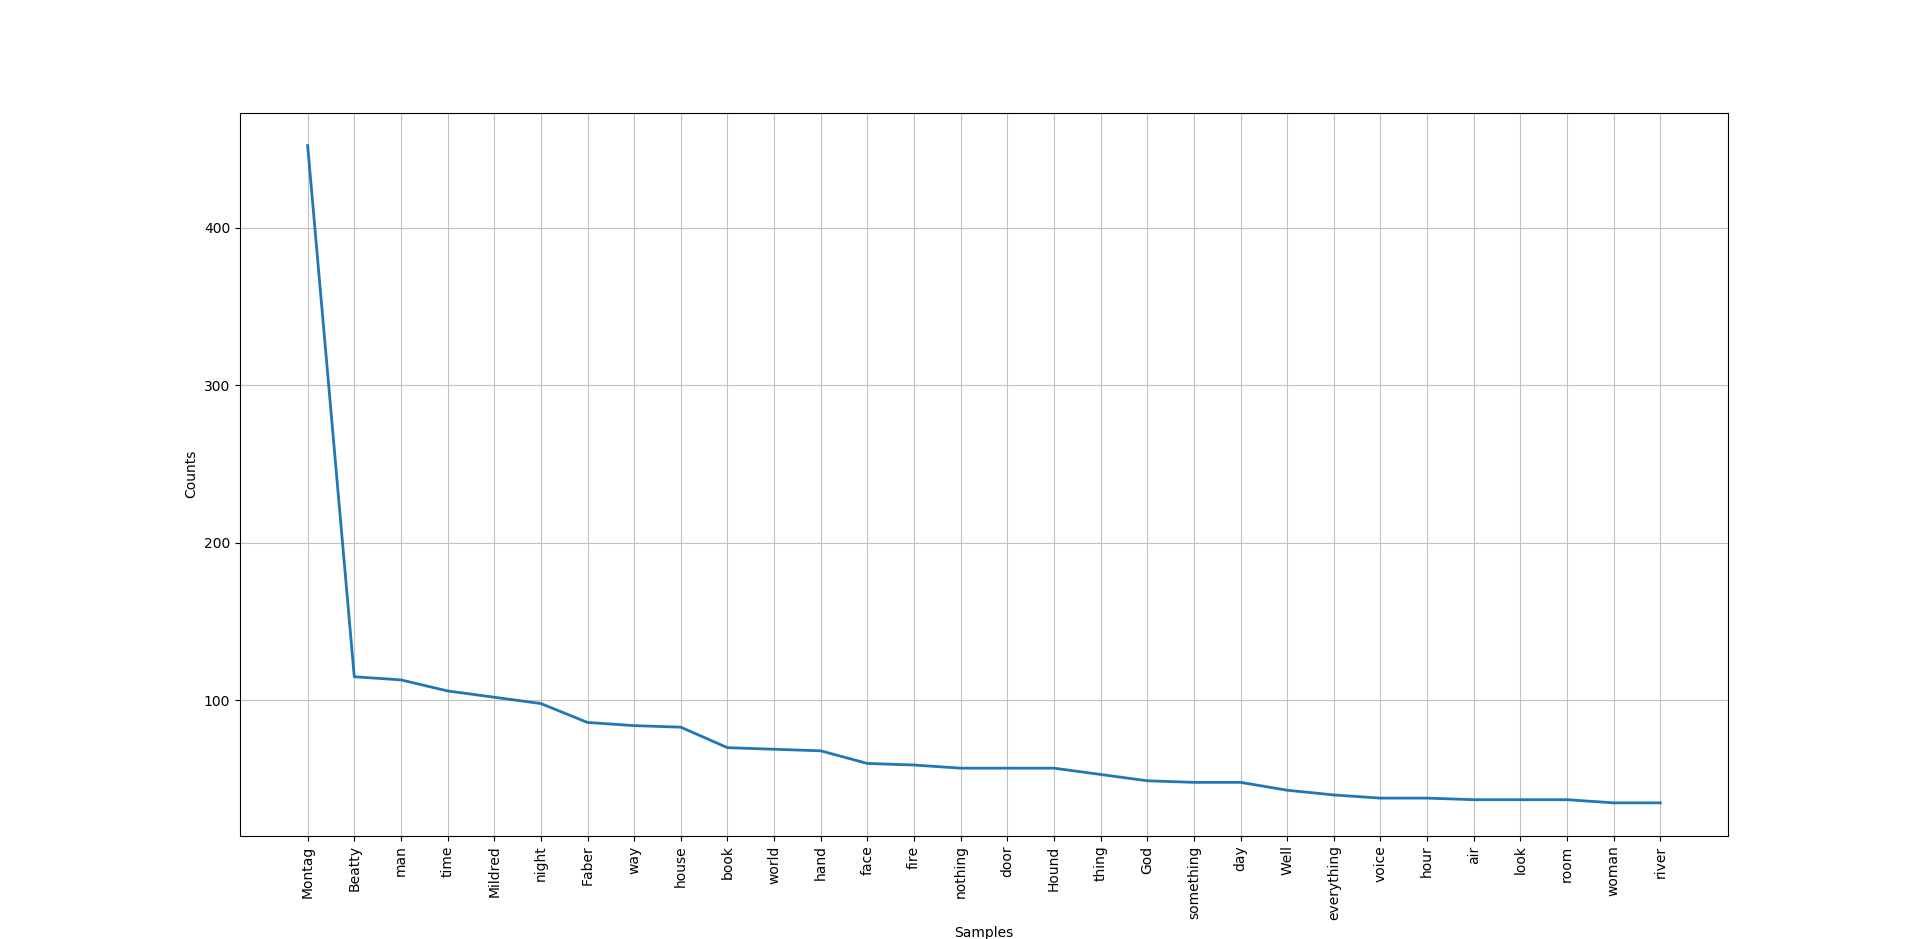
\includegraphics[width=1\linewidth]{fahrenheit_451_nouns}
	\caption{Most used nouns in Fahrenheit 451}\label{fig:fahrenheit_451_nouns}
\end{figure}

\begin{figure}[H]
	\centering
	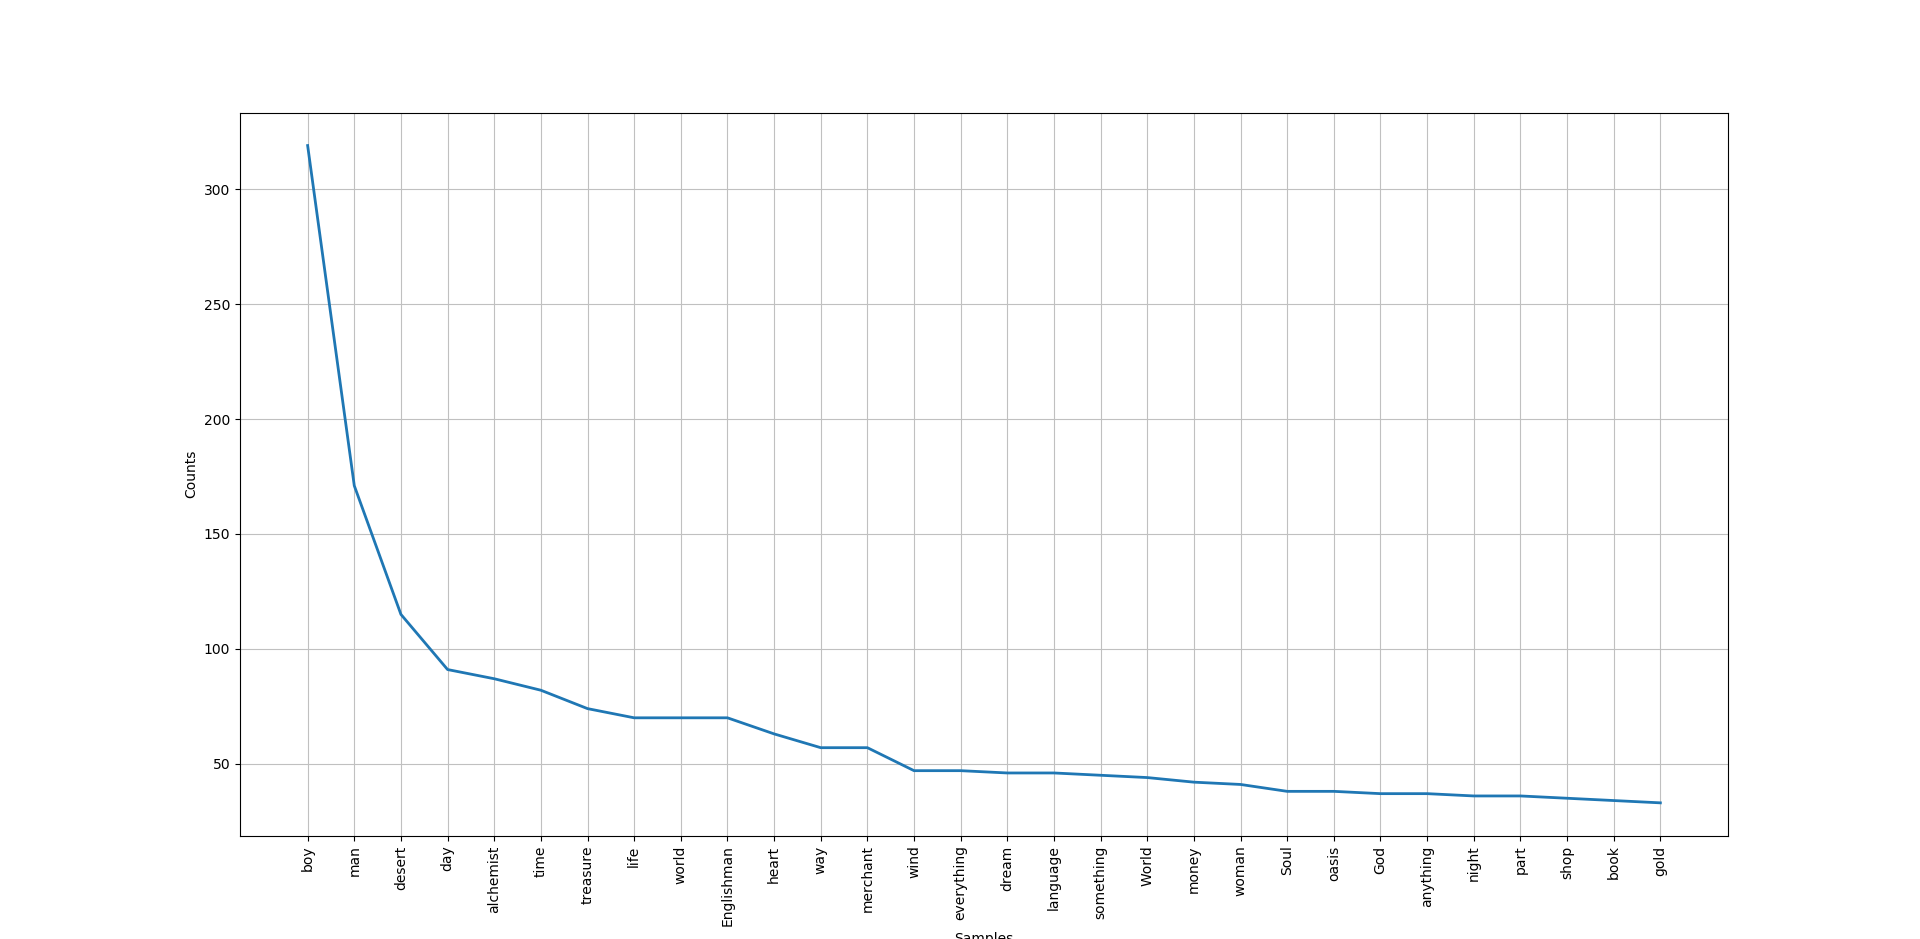
\includegraphics[width=1\linewidth]{the_alchemist_nouns}
	\caption{Most used nouns in The Alchemist}\label{fig:the_alchemist_nouns}
\end{figure}

\begin{figure}[H]
	\centering
	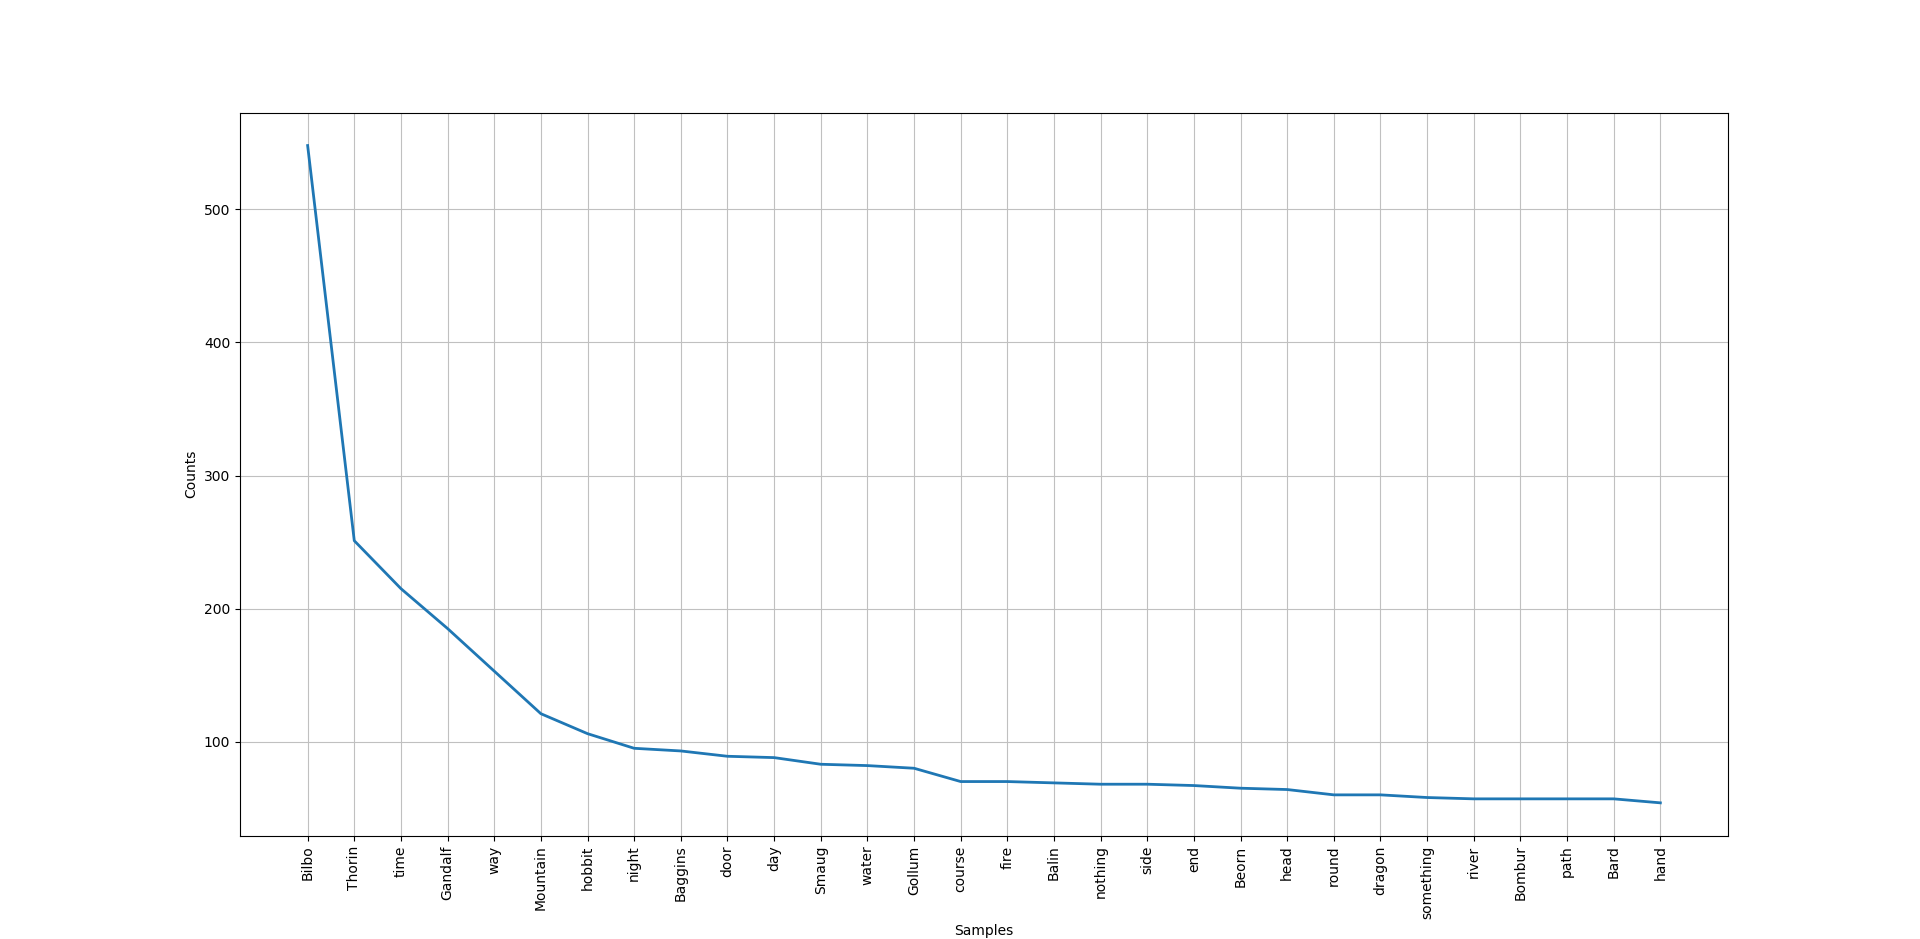
\includegraphics[width=1\linewidth]{the_hobbit_nouns}
	\caption{Most used nouns in The Hobbit}\label{fig:the_hobbit_nouns}
\end{figure}

Our current plan is to use this information to focus summarization around these
important words. The results are not going to be pretty, but at least in some
books it might result in a summary that at least conveys the important plot
points.

\subsection{Evaluation}
Aside from simply reading the summarisation outputs of the algorithm, two
quantitative measures were proposed to evaluate them. It must be noted again
that the scores are expected to be quite low, because the nature of
summarisation leads to very different answers with no objective measure of how
``good'' they are. 

The nltk.translate.bleu\_score toolkit has a function, corpus\_blue, which can
be used for BLEU evaluation. BLEU was originally used for translations, but is
now also used to evaluate summarisations and is based on precision scores of
n-gram overlaps between documents and references. The corpus\_blue allows for
varying weights of 1- to 4-grams, and multiple golden references. 

In table~\ref{table:bleu_huckfinn}, example scores of running this BLEU
evaluation can be seen. In each case, one online summary was evaluated against
the other three as golden references. For pure 1-grams, the scores are always
higher than 2-grams, and indeed they were almost zero for 3- and 4-grams.
Another remark is that while scores over 0.6 seem quite high, the CliffsNotes
score is a low outlier at only 0.295 for the 1-gram case. Finally, it must be
noted that increasing the number of references also increases the score.
Because there are more versions of what a ``correct'' summary is, there is
probably also more overlap of the remaining summary to them. Because it is not
easy to obtain more summaries, the availability of only three to four per book
must simply be kept in mind as a limitation when it comes to evaluation.

\begin{table}[H]
	\centering
	\caption{Example BLEU 1-gram and 2-gram evaluation for online summaries of the Adventures of Huckleberry Finn.}\label{table:bleu_huckfinn}
	\begin{tabular}{l l l }
		\toprule
		\textbf{}   & \textbf{1-gram} & \textbf{2-gram} \\ \midrule
		CliffsNotes & 0.295           & 0.127           \\ \midrule
		SparkNotes  & 0.646           & 0.260           \\ \midrule
		GradeSaver  & 0.655           & 0.262           \\ \midrule
		Wikipedia   & 0.646           & 0.234           \\
		\bottomrule
	\end{tabular}
\end{table}


\section{Conclusions and Anticipated Problems}
In conclusion, our problem seems to be quite hard, and we haven't gotten any
good results yet. We might be able to produce some okay-ish results using
extractive methods, for example by focusing on ``important-character nouns''
that refer to the main characters. However, actually good results are probably
only obtained by state-of-the-art neural network solutions. Specific problems
would be the lack of related work that we can use, and also good datasets.

